%% Application à des données réelles
% le Sweaveopt


\section{Application à des données réelles}

\subsection{Analyse de données}



\begin{frame}{Analyse de données}
Deux jeux de données du paquetage \texttt{CASdatasets} sont utilisés. Soit \texttt{auscathist} et \texttt{nzcathist}.\\~\\ \pause

Historique des catastrophes naturelles pour l'Australie ainsi que pour la Nouvelle-Zélande.
\end{frame}


\begin{frame}
\begin{figure}
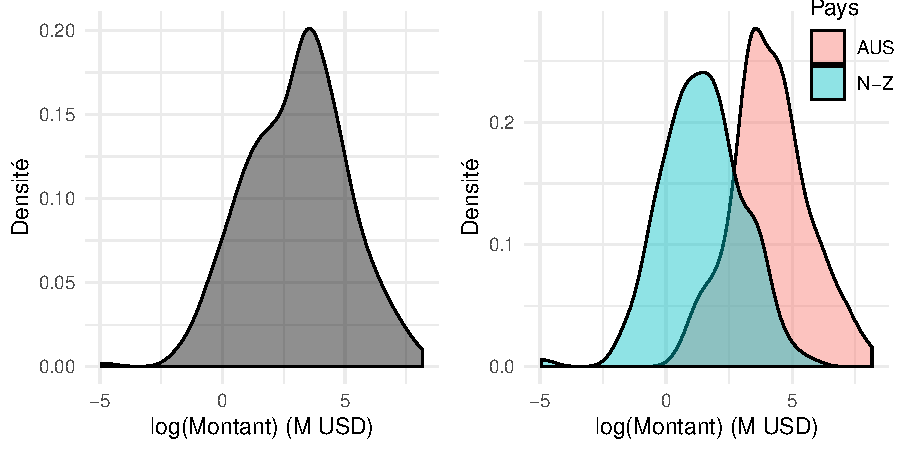
\includegraphics[width=.8\textwidth]{images/fig-005.pdf}
\caption{Densité du logarithme du montant des catastrophes}
\end{figure}
\end{frame}

\begin{frame}
\begin{figure}
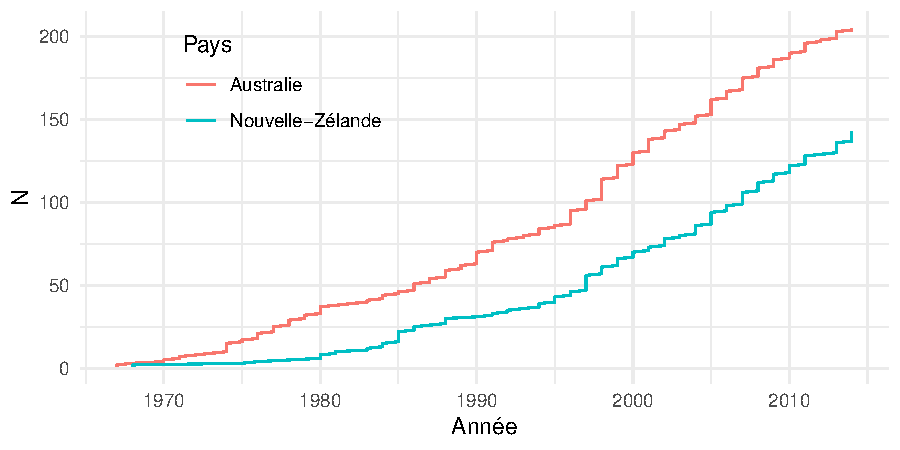
\includegraphics[width=.8\textwidth]{images/fig-006.pdf}
\caption{Nombre cumulatif de catastrophes par pays}
\end{figure}
\end{frame}

\begin{frame}
\begin{figure}
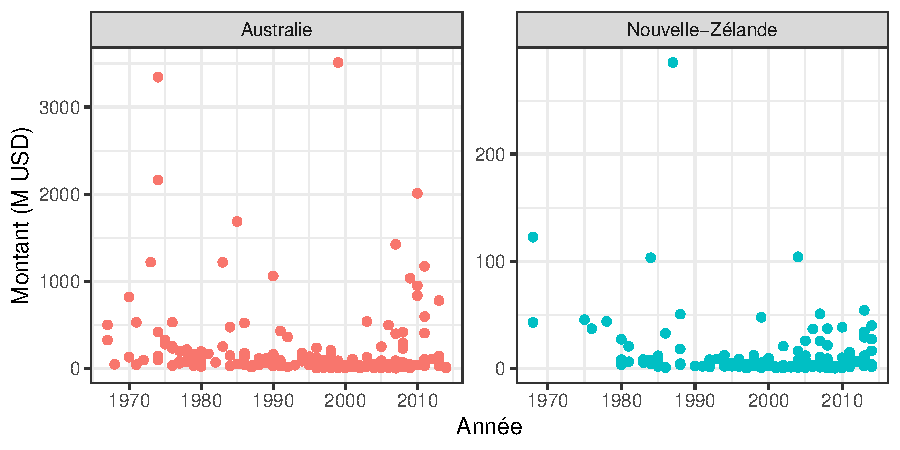
\includegraphics[width=.8\textwidth]{images/fig-007.pdf}
\caption{Évolution des catastrophes par pays}
\end{figure}
\end{frame}


\begin{frame}
% latex table generated in R 3.6.1 by xtable 1.8-4 package
% Tue Dec  3 15:17:43 2019
\begin{table}[ht]
\centering
\begin{tabular}{cccccc}
  \hline
Type & N & Moyenne & Écart & Médiane & Maximum \\ 
  \hline
Bushfire & 26 & 143 & 259 & 39 & 1217 \\ 
  Cyclone & 37 & 325 & 675 & 88 & 3343 \\ 
  Earthquake & 9 & 56 & 91 & 25 & 286 \\ 
  Flood & 83 & 62 & 230 & 5 & 2010 \\ 
  Flood, Storm & 36 & 54 & 79 & 24 & 414 \\ 
  Hailstorm & 41 & 274 & 606 & 75 & 3511 \\ 
  Other & 12 & 121 & 296 & 6 & 1035 \\ 
  Power outage & 2 & 6 & 6 & 6 & 11 \\ 
  Storm & 86 & 97 & 228 & 28 & 1424 \\ 
  Tornado & 12 & 7 & 13 & 3 & 47 \\ 
  Weather & 4 & 11 & 11 & 6 & 27 \\ 
   \hline
\end{tabular}
\caption{Résumé statistique des montants (M USD) par type} 
\label{tab:3.6}
\end{table}\end{frame}

\subsection{Approche classique}

\begin{frame}{Approche classique}
\begin{itemize}
\item Résultats pas montrés de façon détaillée. \pause
\item Approche pas tout à fait adéquate dans le cas présent. \pause
\item Viable, rapide et peut être une bonne solution lorsque seulement les montants sont disponibles. \pause
\item Un seuil de 10 M USD fut sélectionné.
\end{itemize}
\end{frame}

\subsection{Approche dynamique à deux variables}

\begin{frame}{Approche dynamique à deux variables}
\begin{itemize}
\item Année et pays. \pause
\item Variable numérique de temps et variable catégorique à deux niveaux.
\end{itemize}
\end{frame}

\begin{frame}{Paramètre $\rho$}
Le modèle sélectionné pour $\hat\rho$ dépend du pays et du temps:
\begin{equation*}
\log\Bigg(\frac{\hat\rho(x,t)}{1-\hat\rho(x,t)}\Bigg) = \hat{f}_\rho(pays) + \hat{h}^{(2)}_\rho(annee),
\end{equation*}
où ${h}^{(\text{Df})}$ représente une spline naturelle quadratique avec $\text{Df}$ degrés de liberté.
\end{frame}

\begin{frame}
\begin{figure}
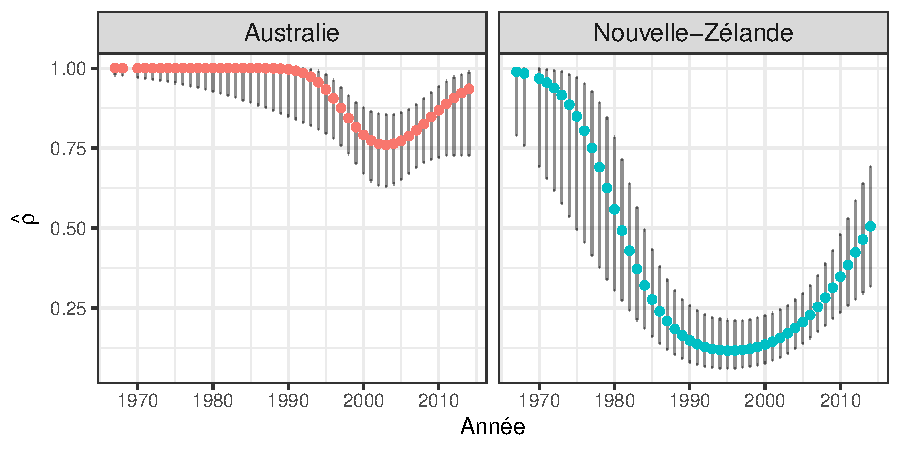
\includegraphics[width=.8\textwidth]{images/fig-013.pdf}
\caption{Prédictions du taux d'excès de seuil}
\end{figure}
\end{frame}


\begin{frame}{Paramètres de la loi Pareto généralisée}
Le modèle sélectionné pour $\hat\xi$ dépend du pays et non du temps:
\begin{equation*}
\hat\xi(x,t) = \hat{f}_\xi(pays).
\end{equation*}
\pause
Le modèle sélectionné pour $\hat\beta$ dépend du pays et du temps:
\begin{equation*}
\hat\beta(x,t) = \hat{f}_\beta(pays) + \hat{h}^{(3)}_\beta(annee).
\end{equation*}
\end{frame}

\begin{frame}
\begin{figure}
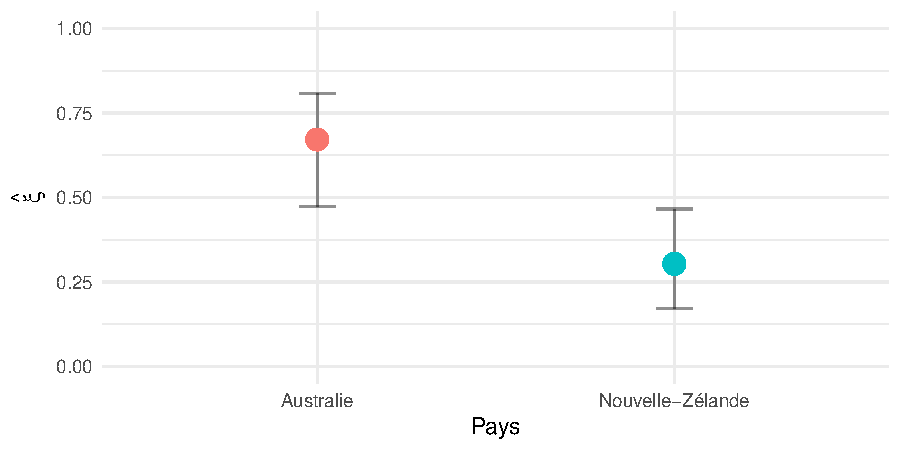
\includegraphics[width=.8\textwidth]{images/fig-015.pdf}
\caption{Prédictions du paramètre $\xi$}
\end{figure}
\end{frame}


\begin{frame}
\begin{figure}
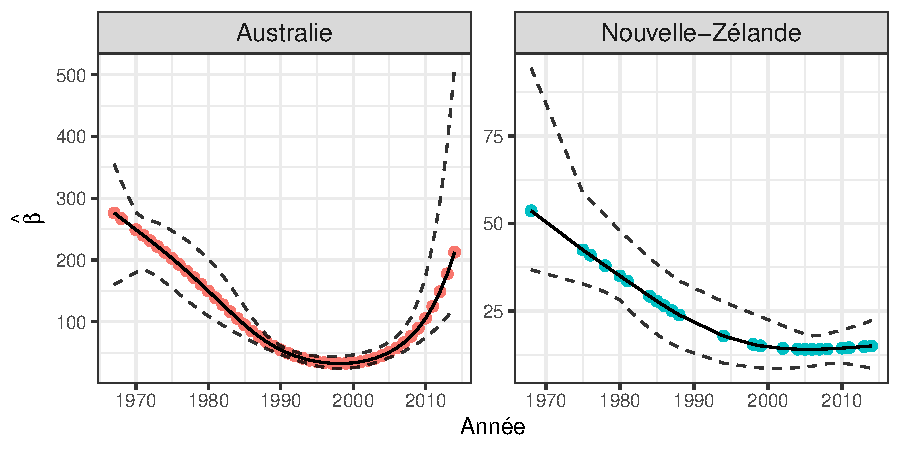
\includegraphics[width=.8\textwidth]{images/fig-016.pdf}
\caption{Prédictions du paramètre $\beta$}
\end{figure}
\end{frame}

\begin{frame}{Validation du modèle}
\begin{figure}
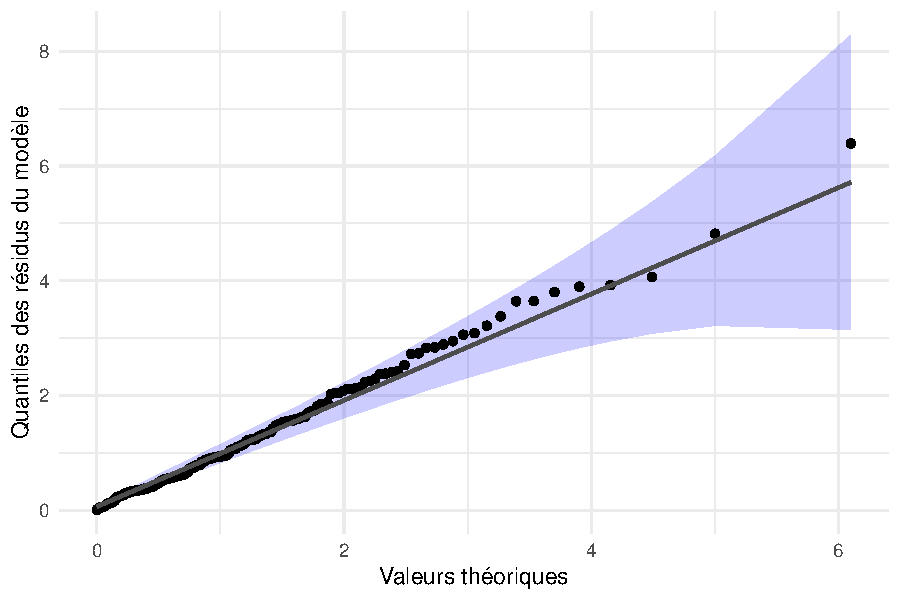
\includegraphics[width=.6\textwidth]{images/fig-018.pdf}
\caption{Graphique \textit{Q-Q} de $\text{Exp}(1)$}
\end{figure}
\end{frame}


\begin{frame}{Mesure \text{VaR}}
\begin{figure}
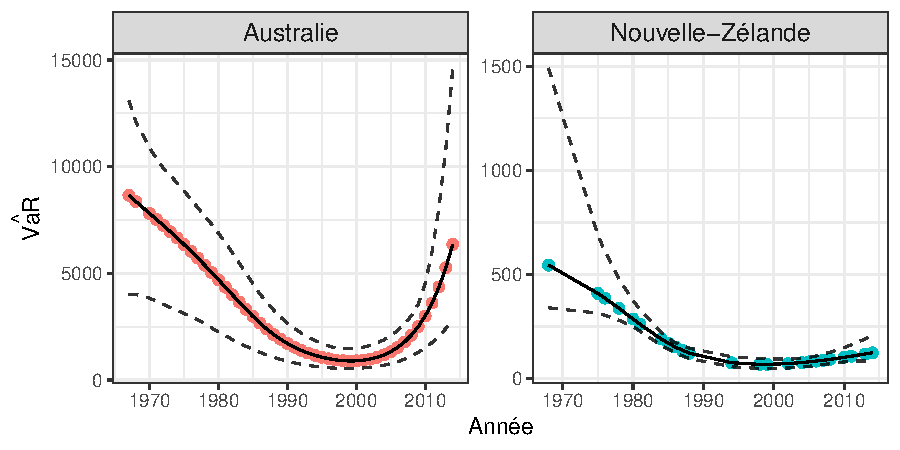
\includegraphics[width=.8\textwidth]{images/fig-019.pdf}
\caption{$\widehat{\text{VaR}_{0.99}}$}
\end{figure}
\end{frame}


\begin{frame}{Résumé}
\begin{itemize}
\item Méthodologie fonctionne. 
\item Donnent les résultats escomptés pour les variables.
\item Amélioration du modèle classique.
\end{itemize}
\end{frame}




\subsection{Approche dynamique à trois variables}

\begin{frame}{Approche dynamique à trois variables}
\begin{itemize}
\item Année, pays et type \pause
\item Regroupement des types.
\end{itemize}
\end{frame}

\begin{frame}
% latex table generated in R 3.6.1 by xtable 1.8-4 package
% Tue Dec  3 15:17:43 2019
\begin{table}[ht]
\centering
\begin{tabular}{cc}
  \hline
Type & Type2 \\ 
  \hline
Bushfire & Bushfire \\ 
  Hailstorm & Hailstorm \\ 
  Cyclone & Cyclone \\ 
  Flood & Flood, Storm \\ 
  Flood, Storm & Flood, Storm \\ 
  Storm & Flood, Storm \\ 
  Other & Other \\ 
  Tornado & Other \\ 
  Earthquake & Other \\ 
  Weather & Other \\ 
  Power outage & Other \\ 
   \hline
\end{tabular}
\caption{Regroupement des types de catastrophes} 
\label{tab:3.7}
\end{table}\end{frame}


\begin{frame}{Paramètre $\rho$}
\begin{equation*}
\log\Bigg(\frac{\hat\rho(x,t)}{1-\hat\rho(x,t)}\Bigg) = \hat{f}_\rho(pays) + \hat{f}_\rho(type) + \hat{h}^{(2)}_\rho(annee)
\end{equation*}
\end{frame}

\begin{frame}
\begin{figure}
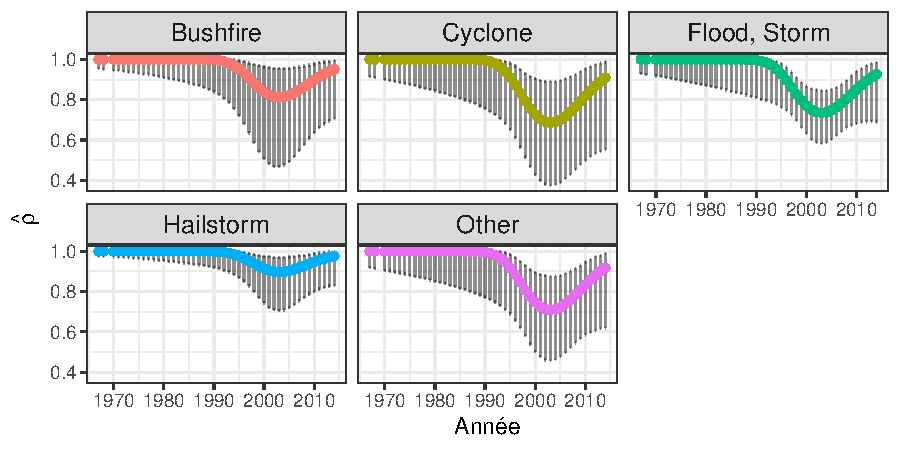
\includegraphics[width=.8\textwidth]{images/fig-023.pdf}
\caption{Prédictions du paramètre $\rho$ pour l'Australie}
\end{figure}
\end{frame}

\begin{frame}
\begin{figure}
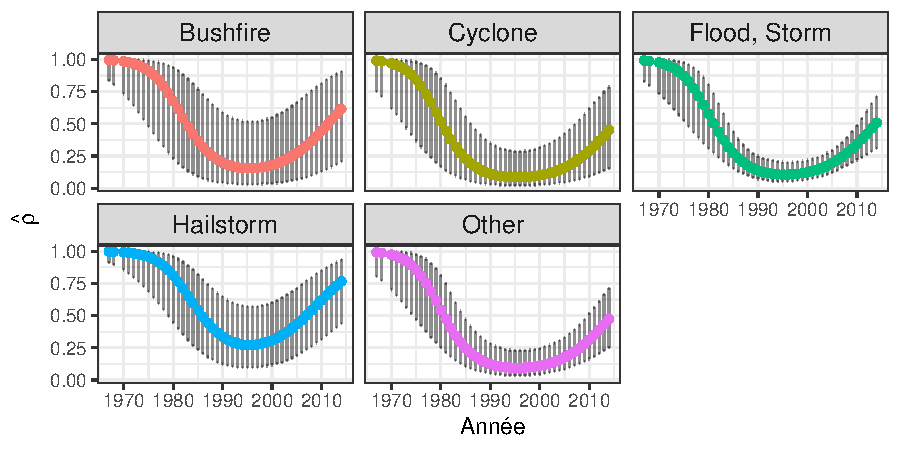
\includegraphics[width=.8\textwidth]{images/fig-024.pdf}
\caption{Prédictions du paramètre $\rho$ pour la Nouvelle-Zélande}
\end{figure}
\end{frame}


\begin{frame}{Paramètres de la loi Pareto généralisée}
\begin{equation*}
\hat\xi(x,t) = \hat{f}_\xi(pays) + \hat{f}_\xi(type)
\end{equation*}
\begin{equation*}
\hat\beta(x,t) = \hat{f}_\beta(pays) + \hat{f}_\xi(type) + \hat{h}^{(4)}_\beta(annee)
\end{equation*}
\end{frame}

\begin{frame}
\begin{figure}
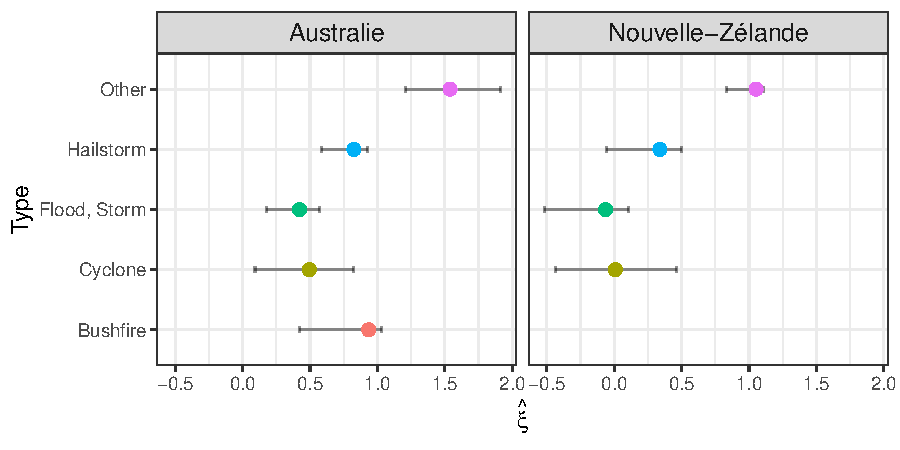
\includegraphics[width=.8\textwidth]{images/fig-026.pdf}
\caption{Prédictions du paramètre $\xi$}
\end{figure}
\end{frame}


\begin{frame}
\begin{figure}
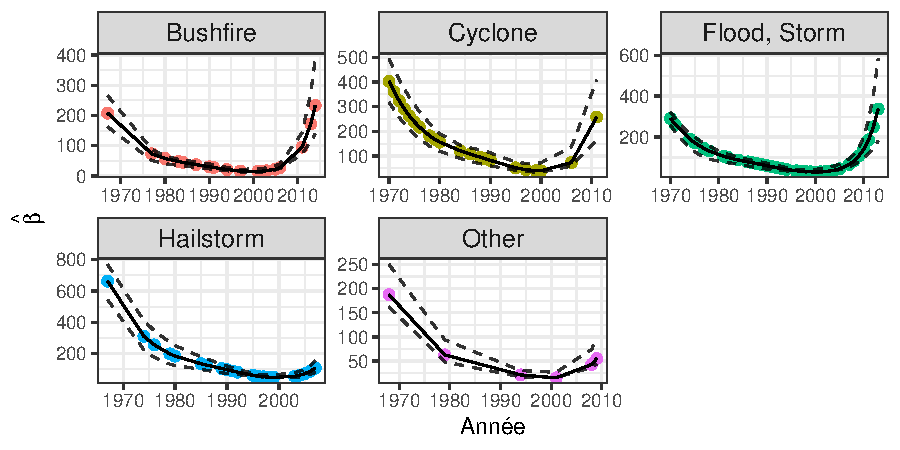
\includegraphics[width=.8\textwidth]{images/fig-027.pdf}
\caption{Prédictions du paramètre $\beta$ pour l'Australie}
\end{figure}
\end{frame}

\begin{frame}
\begin{figure}
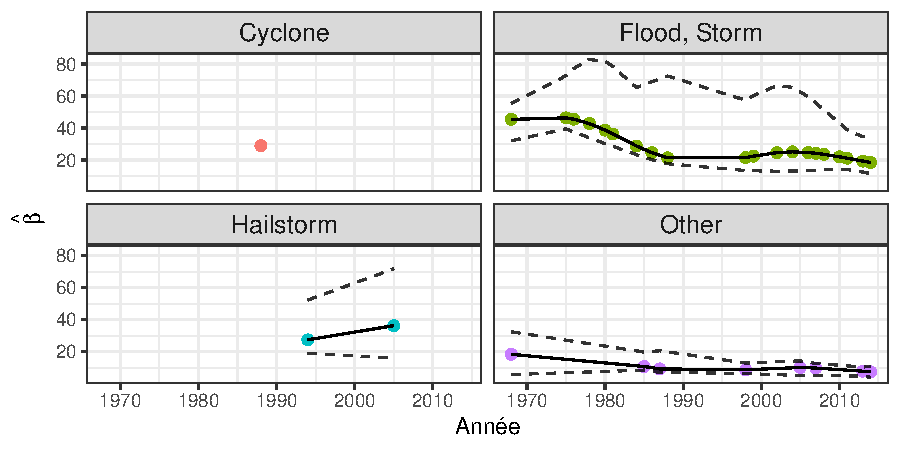
\includegraphics[width=.8\textwidth]{images/fig-028.pdf}
\caption{Prédictions du paramètre $\beta$ pour la Nouvelle-Zélande}
\end{figure}
\end{frame}



\begin{frame}{Validation du modèle}
\begin{figure}
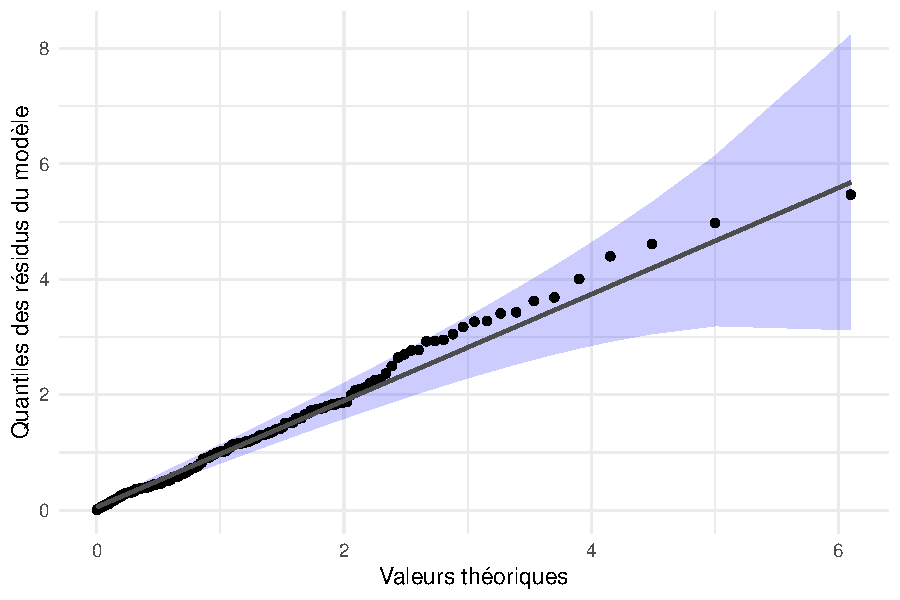
\includegraphics[width=.6\textwidth]{images/fig-030.pdf}
\caption{Graphique \textit{Q-Q} de $\text{Exp}(1)$}
\end{figure}
\end{frame}


\begin{frame}{Mesure \text{VaR}}
\begin{figure}
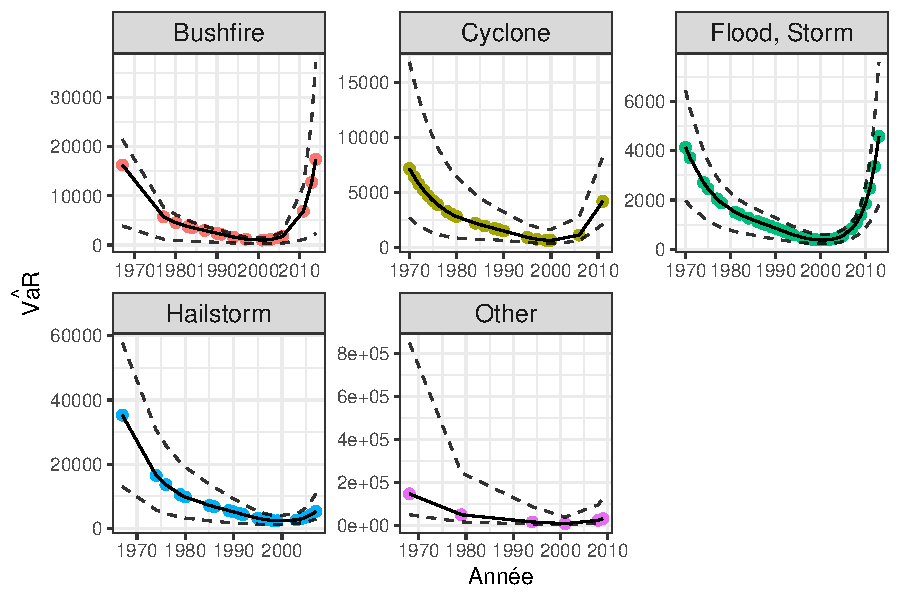
\includegraphics[width=.75\textwidth, height=5.5cm]{images/fig-031.pdf}
\caption{$\widehat{\text{VaR}_{0.99}}$ pour l'Australie}
\end{figure}
\end{frame}

\begin{frame}{Mesure \text{VaR}}
\begin{figure}
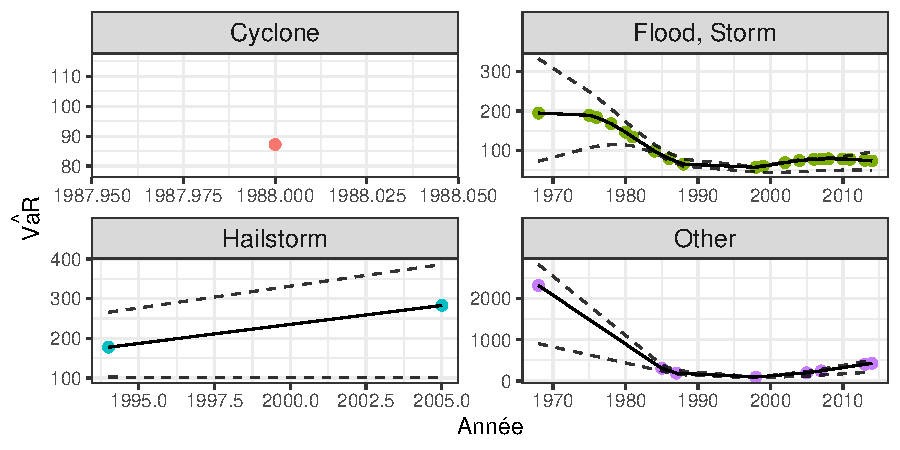
\includegraphics[width=.75\textwidth]{images/fig-032.pdf}
\caption{$\widehat{\text{VaR}_{0.99}}$ pour la Nouvelle-Zélande}
\end{figure}
\end{frame}


\begin{frame}{Résumé}
\begin{itemize}
\item Modèle adéquat. 
\item Aucun gain significatif. 
\item Paramètres et mesures de risques plus volatiles et moins crédibles. 
\end{itemize}
\end{frame}
